%!TEX root=main.tex
% \section{Differentially Private Triangle Counting under the Shuffle Model}
% \section{Triangle Counting}
\section{Triangle Counting Based on Wedge Shuffling}
\label{sec:triangle}
% The existing one-round local triangle algorithms \cite{Imola_USENIX21,Imola_USENIX22,Ye_ICDE20,Ye_TKDE21} suffer from an extremely large estimation error; e.g., when $\epsilon=1$ in edge DP, the relative error is much larger than $1$ in our experiments.
% To address this issue, we propose a differentially private one-round triangle counting algorithm based on wedge shuffling.
Based on our wedge shuffle technique, we first propose a
% differentially private
one-round triangle counting algorithm.
% in the shuffle model.
%
% Section~\ref{sub:challenges} explains technical challenges in our work.
% In particular, we explain why it is challenging to apply the shuffle model to graph data.
Section~\ref{sub:triangle_overview} describes the overview of our algorithms.
Section~\ref{sub:wedge} proposes an algorithm for counting triangles involving a specific user-pair
% proposes a wedge shuffle technique
as a building block of our triangle counting algorithm.
Section~\ref{sub:triangle} proposes
our triangle counting algorithm.
%an algorithm for counting triangles in the entire graph.
% a one-round triangle counting algorithm based on the wedge shuffling.
Section~\ref{sub:var_red} proposes a technique to significantly reduce the variance in our triangle counting algorithm. 
% by ignoring sparse user-pairs.
Section~\ref{sub:summary} summarizes the performance guarantees of our triangle algorithms. 
% The proofs of all statements in this section are given in Appendix~\ref{sec:triangle_proof}.

% \subsection{Technical Challenges}
% \label{sub:challenges}
% The limitation of the one-round local triangle algorithms is an extremely large estimation error.
% This limitation comes from the fact that all three edges are noisy in any noisy edge the data collector can see, as described in Section~\ref{sec:intro}.

% \subsection{Algorithm Overview}
\subsection{Overview}
\label{sub:triangle_overview}
Our wedge shuffle technique tells the data collector the number of common friends of $v_i$ and $v_j$.
However, this information is not sufficient to count triangles in the entire graph.
% the data collector still cannot count triangles, because she does not know whether $v_i$ and $v_j$ are friends.
% To accurately count triangles based on wedge shuffling,
% under the shuffle model,
Therefore, we introduce
% four
three additional techniques:
% strategies:
% \textit{(i) shuffling wedges},
\textit{(i) sending local edges},
% \textit{wedge shuffling},
% \textit{edge sampling without replacement}.
% \textit{sampling independent edges},
% \textit{sampling independent pairs of nodes}.
\textit{(ii) sampling disjoint user-pairs},
% \textit{independent edge sampling},
and
\textit{(iii) variance reduction by ignoring sparse user-pairs}.
% Our wedge shuffle algorithm uses the first and second strategies, whereas our one-round triangle counting algorithm uses the third and fourth strategies.
% Figures~\ref{fig:local_edges} and \ref{fig:triangle_count} show the overview of our wedge shuffle and triangle counting algorithms, respectively.
% the first two strategies and the third strategy, respectively.
Below, we briefly explain each technique.

\begin{figure}[t]
  \centering
  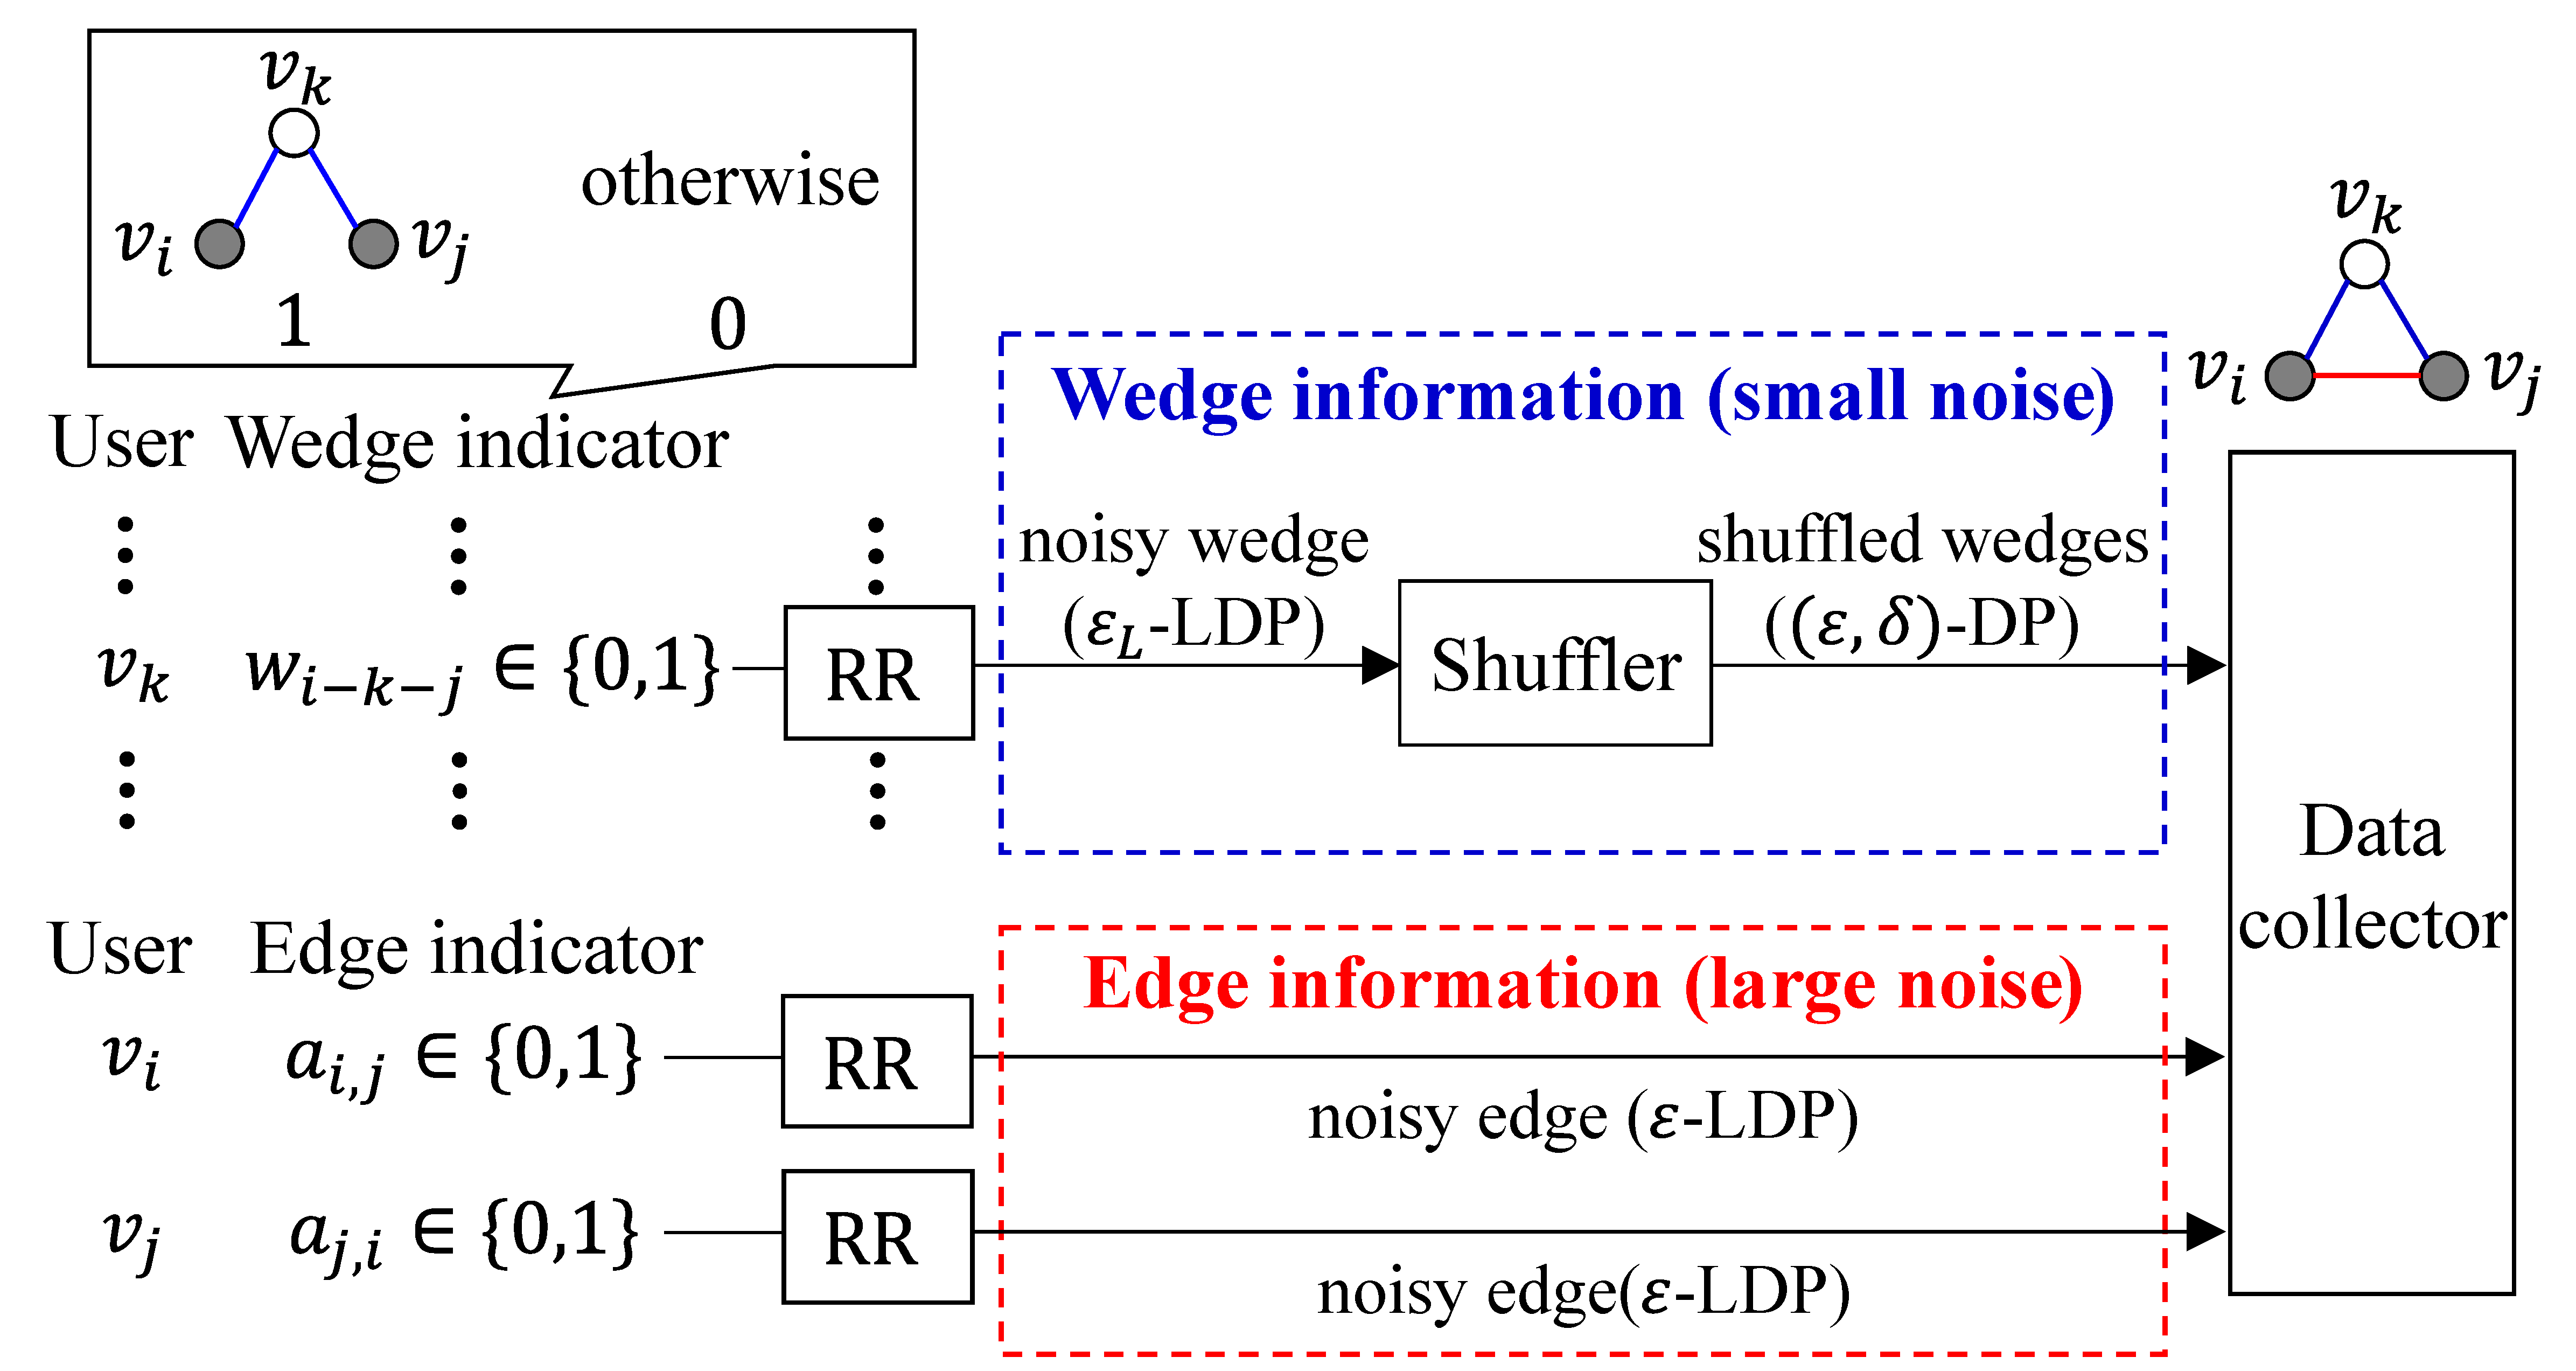
\includegraphics[width=0.99\linewidth]{fig/local_edges.pdf}
  \vspace{-2mm}
  \caption{Overview of our \AlgWSLE{} (Wedge Shuffling with Local Edges) algorithm with inputs $v_i$ and $v_j$.
  %our wedge shuffle algorithm with inputs $v_i$ and $v_j$.
  %(marked with gray).
  }
  \label{fig:local_edges}
% \end{figure}
\vspace{2mm}
% \begin{figure}[t]
  \centering
  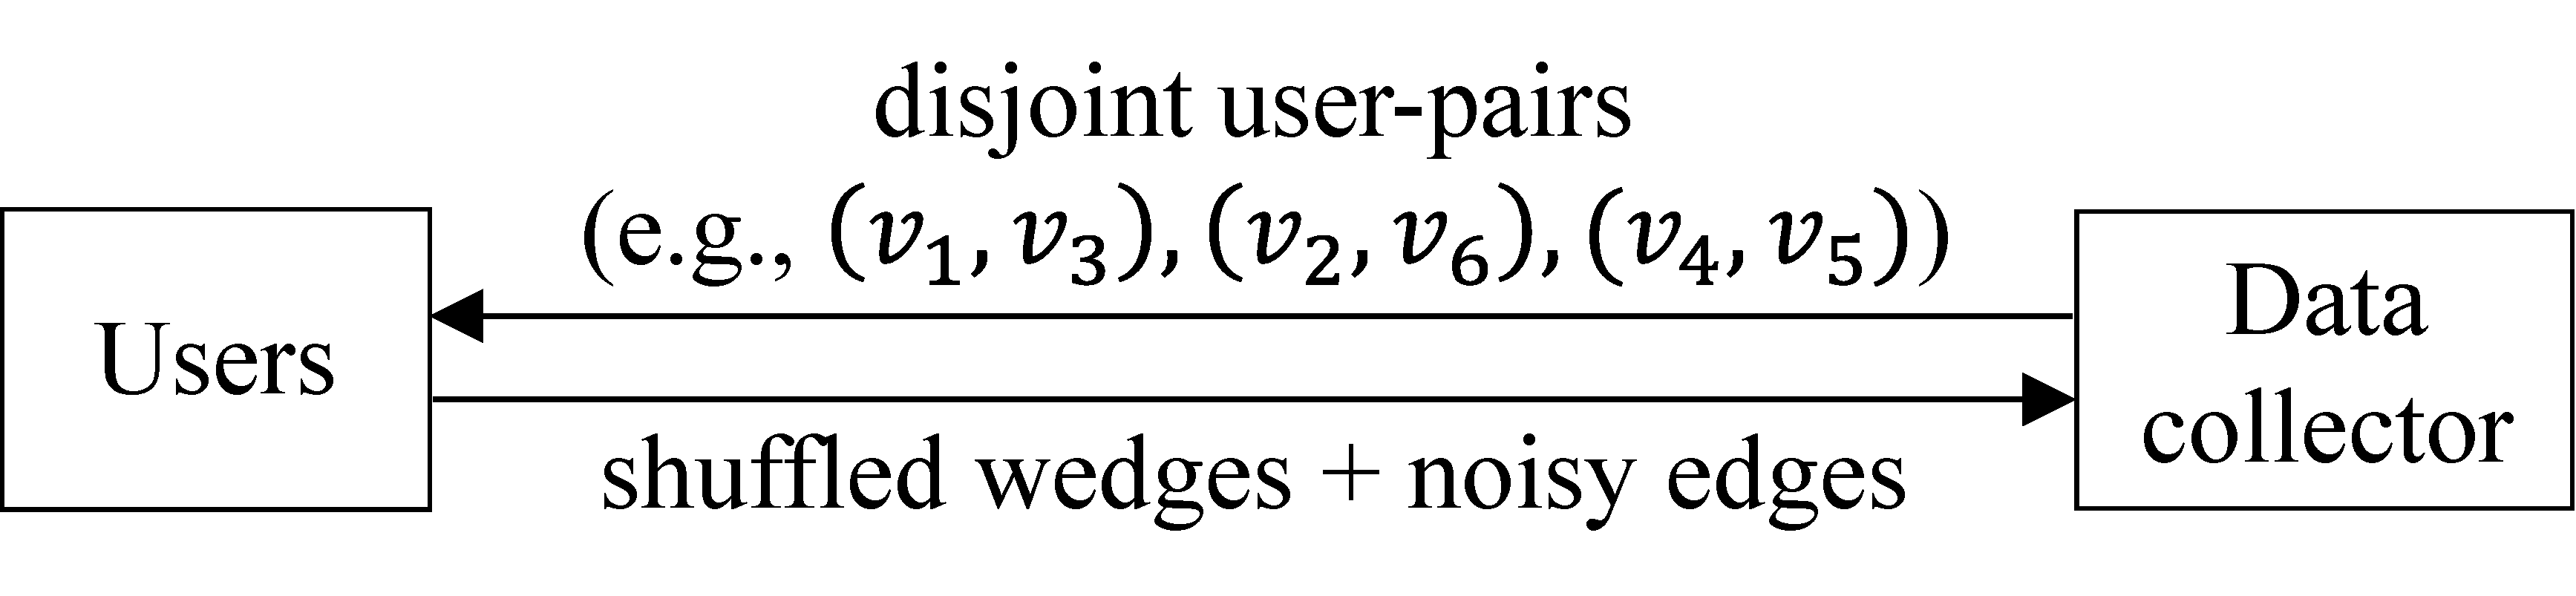
\includegraphics[width=0.7\linewidth]{fig/sampling_pairs2.pdf}
  \vspace{-2mm}
  \caption{Overview of our triangle counting algorithm.
  We use our
  %wedge shuffle
  \AlgWSLE{}
  algorithm with each user-pair.
  %Independent pairs of nodes do share common nodes, e.g., $(v_1, v_3)$, $(v_2, v_6)$, $(v_4, v_5)$.
  }
  \label{fig:triangle_count}
\end{figure}

\smallskip
\noindent{\textbf{Sending Local Edges.}}~~First, we consider the problem of counting triangles involving a specific user-pair $(v_i, v_j)$ and propose an algorithm to send
% The shuffled wedge indicators tell us the number of common friends of $v_i$ and $v_j$.
% However, the data collector still cannot count triangles, because she does not know whether $v_i$ and $v_j$ are friends.
% Thus, our wedge shuffle algorithm sends
\textit{local edges} between $v_i$ and $v_j$, along with shuffled wedges, to the data collector.
We call this the \AlgWSLE{} (Wedge Shuffling with Local Edges) algorithm.
%algorithm \AlgWSLE{} (Wedge Shuffle Edge Local).
% the \textit{wedge shuffling with local edges} algorithm and abbreviate it to \AlgWSLE{}.

Figure~\ref{fig:local_edges} shows the overview of \AlgWSLE{}.
In this algorithm, users $v_i$ and $v_j$ obfuscate edge indicators $a_{i,j}$ and $a_{j,i}$, respectively, using $\epsilon$-RR and send them to the data collector directly (or through the shuffler without shuffling).
%\footnote{It is also possible to send the noisy edge indicators from users $v_i$ and $v_j$ to the data collector through the shuffler. In this case, the shuffler does not shuffle these data.}.
Then, the data collector calculates an unbiased estimate of the triangle count
% from the noisy data.
from the shuffled wedges and the noisy edges.
Because $\epsilon$ is small, a large amount of noise is added to the edge indicators.
However, \textit{only one edge} is noisy (the other two have little noise) in any triangle the data collector sees.
This brings us an advantage over the one-round local algorithms in which all three edges are noisy.

\smallskip
\noindent{\textbf{Sampling Disjoint User-Pairs.}}~~Next, we consider the problem of counting triangles in the entire graph $G$.
A naive solution to this problem is to use our
%wedge shuffling
\AlgWSLE{} algorithm
with all $\binom{n}{2}$ user-pairs as input.
However, it results in very large $\epsilon$ and $\delta$ because it uses each element of the adjacency matrix $\bmA$ many times.
To address this issue,
% To accurately count them under DP,
we propose a triangle counting algorithm that samples
% independent edges (a.k.a. matching), which have no nodes in common.
disjoint user-pairs, ensuring that no user falls in two pairs. 
% which share no common users.
% and then uses the wedge shuffling algorithm for each sampled edge.

Figure~\ref{fig:triangle_count} shows the overview of our triangle algorithm.
The data collector sends the sampled user-pairs to users.
Then, users apply
%our wedge shuffling algorithm
\AlgWSLE{}
with each user-pair
% as input
and send the results to the data collector.
Finally, the data collector calculates an unbiased estimate of the triangle count from the results.
% This can be viewed as edge sampling \cite{Bera_KDD20,Eden_FOCS15,Wu_TKDE16} in triangle counting.
% Edge sampling is known as an efficient sampling method that outperforms other sampling methods such as node sampling and triangle sampling \cite{Wu_TKDE16}.
% Our triangle counting algorithm is also efficient and
% In fact,
Because our triangle algorithm uses each element of
% the adjacency matrix
$\bmA$ \textit{at most once}, it provides $(\epsilon,\delta)$-element DP hence $(2\epsilon,2\delta)$-edge DP.
In addition, our triangle algorithm reduces the time complexity from $O(n^3)$ to $O(n^2)$ by sampling user-pairs rather than using all user-pairs.
% In addition, our wedge shuffle algorithm with a user-pair $(v_i,v_j)$ provides $(\epsilon,\delta)$-DP for each row in the $i$-th and $j$-th columns of the adjacency matrix $\bmA$, and our triangle algorithm samples independent user-pairs.
% Thus, our algorithm provides $(\epsilon,\delta)$-element DP hence $(2\epsilon,2\delta)$-edge DP.

We prove that the MSE of our triangle counting algorithm is
% $O(n^3 d_{max}^2)$.
$O(n^3)$ when we ignore the factor of $d_{max}$.
% when we regard $\epsilon$ and $\delta$ as constants.
When we do not shuffle wedges, the
% expected
MSE is
% $O(n^5)$.
$O(n^4)$.
% This is much smaller than the existing one-round local algorithm with the same time complexity, whose $l_2$ loss is $O(n^5)$, as shown in Section~\ref{sub:upper}.
In addition, the MSE of the existing one-round local algorithm \cite{Imola_USENIX22} with the same time complexity is $O(n^6)$, as proved in
\conference{the full version \cite{Imola_CCSFull22}}\arxiv{
Appendix~\ref{sec:upper}}.
% Section~\ref{sub:upper}.
% Thus, our algorithm has a much smaller estimation error than the local algorithm.
Thus, our
% wedge shuffling
algorithm
provides a dramatic improvement over the local algorithms.

\smallskip
\noindent{\textbf{Variance Reduction.}}~~Although our
% wedge shuffling
algorithm
dramatically
% reduces
improves
the MSE, the factor of $n^3$ may still be large.
Therefore, we propose a variance reduction technique that ignores sparse user-pairs, where either of the two users has a very small degree.
Our basic idea is that the number of triangles involving such a user-pair is very small
% such user-pairs have a very small number of triangles
and can be approximated by $0$.
By ignoring the sparse user-pairs, we can significantly reduce the variance at the cost of introducing a small bias.
We prove that our variance reduction technique reduces the MSE from $O(n^3)$ to $O(n^\gamma)$ where $\gamma\in[2,3)$ and makes one-round triangle counting more accurate.
%accurate one-round triangle counting possible.
% This enables us to accurately count triangles within one round.


% \subsection{Triangle Counting Including a Specific User-Pair}
% \label{sub:triangle_edge}
% \subsection{Wedge Shuffling with Local Edges}
\subsection{WSLE (Wedge Shuffling with Local Edges)}
% \subsection{Sending Local Edges}
\label{sub:wedge}
% Each user $v_k$ ($k \ne i, j$) calculates wedge information $w_{i-k-j} \in \{0,1\}$ that takes $1$ if there is a two-hop path $v_i-v_k-v_j$ and 0 otherwise.
% Then $v_k$ obfuscates $w_{i-k-j}$ using $\epsilon_L$-RR and sends the noisy wedge to the shuffler.
% The shuffler randomly shuffles the noisy wedges to provide $(\epsilon, \delta)$-DP with $\epsilon \ll \epsilon_L$ and sends them to the data collector.
% In addition, users $v_i$ and $v_j$ obfuscate edge information $a_{i,j}$ and $a_{j,i}$, respectively, using $\epsilon$-RR and directly send them to the data collector.

% \smallskip
\noindent{\textbf{Algorithm.}}~~We first
%Consider the problem of counting triangles including a specific user-pair $(v_i,v_j)$.
% To solve this problem, we
propose
% a wedge shuffle algorithm,
the \AlgWSLE{} algorithm
as a building block of our triangle counting algorithm.
\AlgWSLE{} counts
% which estimates the number of
triangles involving a specific user-pair $(v_i,v_j)$.
% We denote this algorithm by \AlgWSLE{}.

Algorithm~\ref{alg:WSLE} shows \AlgWSLE{}.
% This algorithm estimates the number of triangles including a specific user-pair $(v_i,v_j)$.
Let $f_{i,j}^\triangle: \calG \rightarrow \nnints$ be a function that takes $G \in \calG$ as input and outputs the number $f_{i,j}^\triangle(G)$ of triangles involving $(v_i,v_j)$ in $G$.
Let $\hf_{i,j}^\triangle(G) \in \reals$ be an estimate of $f_{i,j}^\triangle(G)$.
% Let $I_{-(i,j)}$ be the set of indices of users other than $v_i$ and $v_j$, i.e., $I_{-(i,j)} = [n]\setminus\{i,j\}$.

\setlength{\algomargin}{5mm}
\begin{algorithm}[t]
  \SetAlgoLined
  \KwData{Adjacency matrix $\bmA \in \{0,1\}^{n \times n}$,
    %Neighbor lists $\bma_1, \ldots, \bma_n \in \{0,1\}^n$,
    %$\epsilon_L \in \nnreals$, $\delta \in [0,1]$, $\epsilon = f(n-2, \epsilon_L, \delta)$,
    $\epsilon \in \nnreals$, $\delta \in [0,1]$,
    user-pair $(v_i,v_j)$.
  }
  \KwResult{Estimate $\hf_{i,j}^\triangle(G)$ of the number $f_{i,j}^\triangle(G)$ of triangles involving $(v_i,v_j)$.}
  %of the count of triangles including $(v_i,v_j)$.}
%   $I_{-(i,j)} \leftarrow [n]\setminus\{i,j\}$\;
%   $q_L \leftarrow \frac{1}{e^{\epsilon_L}+1}$; $q \leftarrow
  %   \frac{1}{e^\epsilon+1}$\;
  $\epsilon_L \leftarrow \texttt{LocalPrivacyBudget}(n,\epsilon,\delta)$\;
%   $\{y_{\pi(k)} | k \in I_{-(i,j)}\} \leftarrow$ \AlgWS{}$(\bmA, \epsilon, \delta, (v_{\sigma(i)}, v_{\sigma(i+1)}))$\;
  \tcc{Wedge shuffling}
  $\{y_{\pi(k)} | k \in I_{-(i,j)}\} \leftarrow$ \AlgWS{}$(\bmA, \epsilon_L, (v_i, v_j))$\;
  \tcc{Send local edges}
%   \For{$i=1$ \KwTo $n$}{
%   \ForEach{$k \in I_{-(i,j)}$}{
%     [$v_k$] $w_{i-k-j} \leftarrow a_{k,i} a_{k,j}$\;
%     [$v_k$] $y_k \leftarrow \calR_{\epsilon_L}^W(x)(w_{i-k-j})$\;
%     [$v_k$] Send $y_k$ to the shuffler\;
%   }
  [$v_i$] $z_i \leftarrow \calR_{\epsilon}^W(x)(a_{i,j})$; Send $z_i$ to the data collector\;
  [$v_j$] $z_j \leftarrow \calR_{\epsilon}^W(x)(a_{j,i})$; Send $z_j$ to the data collector\;
%   \tcc{Shuffler}
%   [s] Sample a random permutation $\pi$ over $I_{-(i,j)}$\;
%   [s] Send $\{y_{\pi(k)} | k \in I_{-(i,j)}\}$ to the data collector\;
  \tcc{Calculate an unbiased estimate}
  [d] $q_L \leftarrow \frac{1}{e^{\epsilon_L}+1}$; $q \leftarrow
  \frac{1}{e^\epsilon+1}$\;
  [d] $\hf_{i,j}^\triangle(G) \leftarrow \frac{(z_i+z_j-2q)\sum_{k \in
  I_{-(i,j)}} (y_{k} - q_L)}{2(1-2q)(1-2q_L)}$\;
  [d] \KwRet{$\hf_{i,j}^\triangle(G)$}
  \caption{\AlgWSLE{}
  %Our wedge shuffle algorithm
  (Wedge Shuffling with Local Edges).
  \AlgWS{} is shown in Algorithm~\ref{alg:WShuffle}.
  %[$v_i$], [s], and [d] represent that the process is run by user $v_i$, the shuffler, and the data collector, respectively.
  % Lines 1 and 2 are run by all parties.
  }\label{alg:WSLE}
\end{algorithm}

% Given $\epsilon$ and $\delta$,
We first call the function \texttt{LocalPrivacyBudget}, which calculates a local privacy budget $\epsilon_L$ from $n$, $\epsilon$, and $\delta$ (line 1).
Specifically, this function calculates $\epsilon_L$
such that $\epsilon$ is a closed-form upper bound (i.e., $\epsilon = f(n-2, \epsilon_L, \delta)$ in (\ref{eq:shuffle_epsilon_f})) or numerical upper bound in the shuffle model with $n-2$ users.
% \cite{Feldman_FOCS21}.
Given $\epsilon_L$, we can easily calculate the closed-form or numerical upper bound $\epsilon$ by (\ref{eq:shuffle_epsilon}) and the open source code in \cite{Feldman_FOCS21}\footnote{\url{https://github.com/apple/ml-shuffling-amplification}.}, respectively.
Thus, we can also easily calculate $\epsilon_L$ from $\epsilon$ by calculating a lookup table for pairs $(\epsilon, \epsilon_L)$ in advance.

Then, we run our wedge shuffle algorithm \AlgWS{} in Algorithm~\ref{alg:WShuffle} (line 2); i.e., each user $v_k \in I_{-(i,j)}$ sends her obfuscated wedge indicator
% obfuscates $w_{i-k-j}$ using $\epsilon_L$-RR $\calR_{\epsilon_L}^W$ and sends the result
$y_k = \calR_{\epsilon_L}^W(w_{i-k-j})$ to the shuffler, and the shuffler sends
shuffled wedge indicators $\{y_{\pi(k)} | k \in I_{-(i,j)}\}$ to the data collector.
%calculates a wedge indicator $w_{i-k-j} \in \{0,1\}$ from her neighbor list $\bma_k$ as follows: $w_{i-k-j} = a_{k,i} a_{k,j}$.
%User $v_k$
% (lines 4-6).
Meanwhile, user $v_i$ obfuscates her edge indicator $a_{i,j}$ using $\epsilon$-RR $\calR_{\epsilon}^W$ and sends the result $z_i = \calR_{\epsilon}^W(a_{i,j})$ to the data collector
% \footnotemark[1]
(line 3).
Similarly, $v_j$ sends $z_j = \calR_{\epsilon}^W(a_{j,i})$ to the data collector (line 4).

% The shuffler samples a uniform random permutation $\pi$ over $I_{-(i,j)}$ and shuffles the wedge indicators based on $\pi$.
% Then, the shuffler sends the shuffled wedge indicators $\{y_{\pi(k)} | k \in I_{-(i,j)}\}$ to the data collector (lines 12-13).

% After receiving $\{y_{\pi(k)} | k \in I_{-(i,j)}\}$, $z_i$, and $z_j$,
Finally, the data collector estimates $f_{i,j}^\triangle(G)$ from $\{y_{\pi(k)} | k \in I_{-(i,j)}\}$, $z_i$, and $z_j$.
% Specifically, let $\hf_{i,j}^\triangle(G) \in \reals$ be an estimate of $f_{i,j}^\triangle(G)$.
Specifically, the data collector calculates the estimate $\hf_{i,j}^\triangle(G)$ as follows:
\begin{align}
    \textstyle{\hf_{i,j}^\triangle(G) = \frac{(z_i+z_j-2q)\sum_{k \in I_{-(i,j)}} (y_{k} -
    q_L)}{2(1-2q)(1-2q_L)},}
    \label{eq:hfij_triangle}
\end{align}
where $q_L = \frac{1}{e^{\epsilon_L}+1}$ and $q = \frac{1}{e^\epsilon+1}$ (lines 5-6).
Note that this estimate involves simply summing over the set $\{y_{\pi(k)}\}$ and does not require knowing the value of $\pi$. This is
consistent with the shuffle model.
As we prove later, $\hf_{i,j}^\triangle(G)$ in (\ref{eq:hfij_triangle}) is an unbiased estimate of $f_{i,j}^\triangle(G)$.

\smallskip
\noindent{\textbf{Theoretical Properties.}}~~Below, we show some theoretical properties of \AlgWSLE{}.
% First, we prove that \AlgWSLE{} provides DP:
% \begin{theorem}
% \label{thm:DP_I}
% \AlgWSLE{} provides $(\epsilon, \delta)$-element DP and $(2\epsilon, 2\delta)$-edge DP.
% \end{theorem}
% Intuitively, Theorem~\ref{thm:DP_I} comes from the fact that \AlgWSLE{} uses only the $i$-th and $j$-th columns of the adjacency matrix $\bmA$ and protects each element with $(\epsilon,\delta)$-DP.
% See Appendix~\ref{sec:triangle_proof} for details.
%
% Next,
First, we prove that
the estimate $\hf_{i,j}^\triangle(G)$
% of \AlgWSLE{}
is unbiased:
\begin{theorem}
\label{thm:unbiased_I}
  For any indices $i,j \in [n]$, the estimate produced by
  $\AlgWSLE{}$ satisfies $\E[\hf_{i,j}^\triangle(G)] = f_{i,j}^\triangle(G)$.
% \AlgWSLE{} provides an unbiased estimate, i.e.,
% \begin{align*}
% \E[\hf_{i,j}^\triangle(G)] = f_{i,j}^\triangle(G).
% \end{align*}
\end{theorem}

% Finally,
Next,
we show the MSE ($=$ variance). 
% of \AlgWSLE{}.
% $\hf_{i,j}^\triangle(G)$.
Recall that in the shuffle model, $\epsilon_L = \log n + O(1)$ when $\epsilon$ and $\delta$ are constants.
%see Section~\ref{sub:shuffle}
We show
% the expected $l_2$ losses for a general case and the case where $\epsilon_L = \Theta(\log n)$:
the MSE for a general case and for the shuffle model:
\begin{theorem}
\label{thm:l2-loss_I}
  For any indices $i,j \in [n]$, the estimate produced by
  \AlgWSLE{} provides the following utility guarantee:
% In \AlgWSLE{},
\begin{align}
& \MSE(\hf_{i,j}^\triangle(G)) = \V[\hf_{i,j}^\triangle(G)] \nonumber\\
  & \leq \frac{n q_L + q(1-2q_L)^2 d_{max}^2}{(1-2q)^2(1-2q_L)^2} \triangleq
  err_{\AlgWSLE}(n,d_{max},q,q_L).
\label{eq:l2_I_general}
\end{align}
  When $\epsilon$ and $\delta$ are constants and $\epsilon_L = \log n + O(1)$, we
  have
\begin{align}
  & err_{\AlgWSLE{}}(n,d_{max}, q, q_L) = O(d_{max}^2).
\label{eq:l2_I_shuffle}
\end{align}
\end{theorem}
The equation (\ref{eq:l2_I_shuffle}) follows from (\ref{eq:l2_I_general}) because $q_L = \frac{1}{e^{\epsilon_L}+1} = \frac{1}{n e^{O(1)} + 1}$. 
% Theorem~\ref{thm:l2-loss_I} states that
Because \AlgWSLE{} is a building block for our triangle counting algorithms, we
introduce the notation $err_{\AlgWSLE{}}(n,d_{max}, q, q_L)$ for our upper bound
in~\eqref{eq:l2_I_general}. Observing
\eqref{eq:l2_I_general}, if we do not use the shuffling technique (i.e.,
$\epsilon_L = \epsilon$), then $err_{\AlgWSLE{}}(n,d_{max}, q, q_L) = O(n + d_{max}^2)$ when we
treat $\epsilon$ and $\delta$ as constants.
In contrast, in the shuffle model where we have $\epsilon_L = \log n + O(1)$,
then $err_{\AlgWSLE{}}(n,d_{max}, q, q_L) = O(d_{max}^2)$.
This means that wedge shuffling reduces the MSE from $O(n + d_{max}^2)$ to $O(d_{max}^2)$, which is significant when $d_{max} \ll n$.

% \subsection{Triangle Counting Based on Wedge Shuffle}
% \subsection{Wedge Shuffle-Based Triangle Counting}
% \subsection{WSLE-Based Triangle Counting}
\subsection{Triangle Counting}
% \subsection{Sampling Independent User-Pairs}
\label{sub:triangle}
\noindent{\textbf{Algorithm.}}~~Based on
%Now, we turn our attention to the problem of counting triangles in the entire graph $G$ and propose a triangle counting algorithm
% Our wedge shuffle algorithm \AlgWSLE{} estimates the number of triangles including a specific user-pair $(v_i,v_j)$.
% Based on
% this,
\AlgWSLE{},
we propose an algorithm that counts triangles in the entire graph $G$.
We denote this algorithm by \AlgWSTri{}, as it applies wedge shuffling to triangle counting.

Algorithm~\ref{alg:wshuffle_triangle} shows \AlgWSTri{}.
First, the data collector samples disjoint user-pairs, 
ensuring that no user falls in two pairs. 
% which share no common users.
Specifically, it calls the function \texttt{RandomPermutation}, which samples a uniform random permutation $\sigma$ over $[n]$ (line 1).
Then, it samples disjoint user-pairs as
$(v_{\sigma(1)}, v_{\sigma(2)}), (v_{\sigma(3)}, v_{\sigma(4)}), \ldots, (v_{\sigma(2t-1)}, \allowbreak v_{\sigma(2t)})$, where $t \in [\lfloor \frac{n}{2} \rfloor]$.
The parameter $t$ represents the number of user-pairs and controls the trade-off between the MSE and the time complexity;
when $t = \lfloor \frac{n}{2} \rfloor$, the MSE is minimized and the time complexity is maximized.
The data collector sends the sampled user-pairs to users (line 2).

\setlength{\algomargin}{5mm}
\begin{algorithm}[t]
  \SetAlgoLined
  \KwData{Adjacency matrix $\bmA \in \{0,1\}^{n \times n}$, $\epsilon \in \nnreals$, $\delta \in [0,1]$, $t \in [\lfloor \frac{n}{2} \rfloor]$.
  }
  \KwResult{Estimate $\hf^\triangle(G)$ of $f^\triangle(G)$.}
%   \tcc{Data collector}
  \tcc{Sample disjoint user-pairs}
  [d] $\sigma \leftarrow$\texttt{RandomPermutation}$(n)$\;
  [d] Send $(v_{\sigma(1)}, v_{\sigma(2)}), \ldots, (v_{\sigma(2t-1)}, v_{\sigma(2t)})$ to users\;
%  \ForEach{$i \in \{1, 3, \ldots, 2t-1\}$}{
%    [$d$] Send $(\sigma(i), \sigma(i+1))$ to users\;
%  }
%   \tcc{Users, shuffler, and data collector}
%   \tcc{Wedge shuffling with local edges}
  \ForEach{$i \in \{1, 3, \ldots, 2t-1\}$}{
    $\hf_{\sigma(i), \sigma(i+1)}^\triangle(G) \leftarrow$ \AlgWSLE{}$(\bmA, \epsilon, \delta, (v_{\sigma(i)}, v_{\sigma(i+1)}))$\;
  }
%   \tcc{Data collector}
  \tcc{Calculate an unbiased estimate}
  [d] $\hf^\triangle(G) \leftarrow \frac{n(n-1)}{6t} \sum_{i=1, 3, \ldots, 2t-1} \hf_{\sigma(i),\sigma(i+1)}^\triangle(G)$\;
  [d] \KwRet{$\hf^\triangle(G)$}
  \caption{Our triangle counting algorithm \AlgWSTri{}.
  %Our wedge shuffle-based triangle counting algorithm \AlgWSTri{}.
  %[d] represents that the process is run by the data collector.
  \AlgWSLE{} is shown in Algorithm~\ref{alg:WSLE}.
  }\label{alg:wshuffle_triangle}
\end{algorithm}

Then, we run our wedge algorithm \AlgWSLE{} in Algorithm~\ref{alg:WSLE} with each sampled user-pair as input (lines 3-5).
Finally, the data collector estimates the triangle count $f^\triangle(G)$ as follows:
\begin{align}
    \textstyle{\hf^\triangle(G) = \frac{n(n-1)}{6t} \sum_{i=1, 3, \ldots, 2t-1} \hf_{\sigma(i),\sigma(i+1)}^\triangle(G)}
   \label{eq:hf_triangle_II}
\end{align}
(line 6). 
Note that a single triangle is never counted by more than one user-pair, as the user-pairs never overlap. 
Later, we prove that $\hf^\triangle(G)$ in (\ref{eq:hf_triangle_II}) is unbiased.

\smallskip
\noindent{\textbf{Theoretical Properties.}}~~We prove that
% our triangle counting algorithm
\AlgWSTri{} provides DP:
% Below, we show the privacy and utility of \AlgWSTri{}.
% We first prove that \AlgWSTri{} provides DP:
\begin{theorem}
\label{thm:DP_II}
\AlgWSTri{} provides $(\epsilon, \delta)$-element DP and $(2\epsilon, 2\delta)$-edge DP.
\end{theorem}
Theorem~\ref{thm:DP_II} comes from the fact that
\AlgWSLE{} with a user-pair $(v_i,v_j)$ provides $(\epsilon,\delta)$-DP for each element in the $i$-th and $j$-th columns of the adjacency matrix $\bmA$ and that \AlgWSTri{} samples disjoint user-pairs, i.e., it uses each element of $\bmA$ at most once.
% and protect each element with $(\epsilon,\delta)$-DP.

Note that running \AlgWSLE{} with all $\binom{n}{2}$ user-pairs 
% requires a very large privacy budget --
% By composition,
% it 
provides $((n-2) \epsilon, (n-2) \delta)$-DP, as it uses each element of $\bmA$ at most $n-2$ times.
The privacy budget is very large, even using the advanced composition \cite{DP,Kairouz_ICML15}.
We avoid this issue by sampling user-pairs that share no common users.

We also prove that
% the estimate of \AlgWSTri{} is unbiased:
\AlgWSTri{} provides an unbiased estimate:
% Next, we show the utility of \AlgWSTri{}:
\begin{theorem}
\label{thm:unbiased_II}
The estimate produced by \AlgWSTri{} satisfies $\allowbreak \E[\hf^\triangle(G)] = f^\triangle(G)$.
% \AlgWSTri{} provides an unbiased estimate, i.e.,
% \begin{align*}
% \E[\hf^\triangle(G)] = f^\triangle(G).
% \end{align*}
\end{theorem}

Next, we analyze the MSE ($=$ variance) of \AlgWSTri{}.
This analysis is 
% complicated 
non-trivial 
because \AlgWSTri{} samples each user-pair \textit{without replacement}.
In this case, the sampled user-pairs are not independent.
However, we can prove that
$t$ estimates in (\ref{eq:hf_triangle_II}) are negatively correlated with each other (\conference{see the full version \cite{Imola_CCSFull22} for details}\arxiv{Lemma~\ref{lem:sampling_replacement_var} in Appendix~\ref{sub:l2-loss_II_proof}}).
%the covariance of two estimates $\hf_{\sigma(i),\sigma(i+1)}^\triangle(G)$ and $\hf_{\sigma(j),\sigma(j+1)}^\triangle(G)$ in (\ref{eq:hf_triangle_II})
Thus, the variance of the sum of $t$ estimates
%$\sum_{i=1, 3, \ldots, 2t-1} \hf_{\sigma(i),\sigma(i+1)}^\triangle(G)$
in (\ref{eq:hf_triangle_II}) is upper bounded by the sum of their variances, each of which is given by Theorem~\ref{thm:l2-loss_I}.
This brings us to the following result:

\begin{theorem}
\label{thm:l2-loss_II}
The estimate produced by \AlgWSTri{} provides the following utility guarantee:
\begin{align}
& \MSE(\hf^\triangle(G)) = \V[\hf^\triangle(G)] \nonumber\\
  &\leq
  \frac{n^4}{36t}err_{\AlgWSLE{}}(n,d_{max},q,q_L) +
  \frac{n^3}{36t}d_{max}^3, \label{eq:thm:l2_II}
\end{align}
where $err_{\AlgWSLE{}}(n,d_{max},q,q_L)$ is given by (\ref{eq:l2_I_general}).
  When $\epsilon$ and $\delta$ are constants,  $\epsilon_L = \log(n) + O(1)$, and
  $t = \lfloor\frac{n}{2}\rfloor$, we have
\begin{align}
\MSE(\hf^\triangle(G))
  &\leq
  O(n^3d_{max}^2). \label{eq:thm:l2_II_simp}
\end{align}
\end{theorem}
% Theorem~\ref{thm:unbiased_II} states that the estimate of \AlgWSTri{} is unbiased.

The inequality (\ref{eq:thm:l2_II_simp}) follows from (\ref{eq:l2_I_shuffle}) and (\ref{eq:thm:l2_II}). 
The first and second terms in~(\ref{eq:thm:l2_II}) are caused by
% the randomness in
Warner's RR
% for local edges
and the sampling of disjoint user-pairs, respectively.
In other words, the MSE of \AlgWSTri{} can be decomposed into two factors: the RR
% for local edges
and user-pair sampling.

For example, assume that $t = \lfloor \frac{n}{2} \rfloor$.
When we do not shuffle wedges (i.e., $\epsilon_L = \epsilon$), then
$err_{\AlgWSLE{}}(n,d_{max},q,q_L) = O(n + d_{max}^2)$, and
MSE in (\ref{eq:thm:l2_II}) is $O(n^4 + n^3 d_{max}^2)$.
When we shuffle wedges, the MSE is $O(n^3 d_{max}^2)$.
Thus, when we ignore the factor of $d_{max}$, our wedge shuffle technique reduces the MSE from $O(n^4)$ to $O(n^3)$ in triangle counting.
The factor of $n^3$ is caused by the RR for local edges.
This is intuitive because a large amount of noise is added to the local edges.

Finally, we analyze the time complexity of \AlgWSTri{}.
The time complexity of running \AlgWSLE{} with all $\binom{n}{2}$ user-pairs is $O(n^3)$, as there are $O(n^2)$ user-pairs in total and \AlgWSLE{} requires the time complexity of $O(n)$.
In contrast, the time complexity of \AlgWSTri{} with $t = \lfloor \frac{n}{2} \rfloor$ is $O(n^2)$ because it samples $O(n)$ user-pairs.
Thus, \AlgWSTri{} reduces the time complexity from $O(n^3)$ to $O(n^2)$ by user-pair sampling.
We can further reduce the time complexity at the cost of increasing the MSE by setting $t$ small,
% the number $t$ of sampled user-pairs small,
i.e., $t \ll \lfloor \frac{n}{2} \rfloor$.
% However, it comes at the cost of increasing the $l_2$ loss.

% \subsection{Variance Reduction Based on Ignoring Sparse User-Pairs}
\subsection{Variance Reduction}
\label{sub:var_red}
\noindent{\textbf{Algorithm.}}~~\AlgWSTri{}
% Our triangle counting algorithm \AlgWSTri{}
achieves the MSE of $O(n^3)$ when we ignore the factor of $d_{max}$.
% However, the factor of $n^3$ is still large because the square of the true count $f^\triangle(G)$ is $O(n^2)$.
% To provide a small relative error, we want to reduce the $l_2$ loss of \AlgWSTri{} from $O(n^3)$ to at most $O(n^2)$.
% To this end,
To provide a smaller estimation error,
we propose a variance reduction technique that ignores sparse user-pairs.
We denote our triangle counting algorithm with the variance reduction technique by \AlgWSTriVR{}.

% Let $d_{i,j} = \min\{d_i, d_j\}$ be the minimum degree of users $v_i$ and $v_j$.
As explained in Section~\ref{sub:triangle}, the factor of $n^3$ is caused by the RR for local edges.
However, most user-pairs $v_i$ and $v_j$ have a very small minimum degree
% $d_{i,j} \ll d_{max}$,
$\min\{d_i, d_j\} \ll d_{max}$,
and there is no edge $(v_i, v_j)$ between them in almost all cases.
In addition, even if there is an edge $(v_i, v_j)$, the number of triangles involving the sparse user-pair is very small
% (at most $d_{i,j}-1$)
(at most $\min\{d_i, d_j\}$)
and can be approximated by $0$.
% Thus,
% we can approximate the number of triangles including the sparse user-pair by $0$.
By ignoring such sparse user-pairs, we can dramatically reduce the variance of the RR for local edges at the cost of a small bias.
This is an intuition behind our variance reduction technique.

% Specifically, we consider the following improvement of \AlgWSTri{}.
% Let $d_{i,j} = \min\{d_i, d_j\}$ be the minimum degree of users $v_i$ and $v_j$.
% Below, we assume that the data collector knows each user $v_i$'s degree $d_i$ for ease of explanation.
% Note that $d_i$ can leak the information about edges of $v_i$.
% Thus, we explain how to privately estimate $d_i$ with edge DP within one-round at the end of Section~\ref{sub:var_red}.
Algorithm~\ref{alg:wshuffle_triangle_vr} shows \AlgWSTriVR{}.
This algorithm detects sparse user-pairs based on the degree information.
However, user $v_i$'s degree $d_i$ can leak the information about edges of $v_i$.
Thus, \AlgWSTriVR{} calculates a differentially private estimate of $d_i$ within one round.

\setlength{\algomargin}{5mm}
\begin{algorithm}[t]
  \SetAlgoLined
  \KwData{Adjacency matrix $\bmA \in \{0,1\}^{n \times n}$, $\epsilon_1, \epsilon_2 \in \nnreals$, $\delta \in [0,1]$, $t \in [\lfloor \frac{n}{2} \rfloor]$, $c \in \nnreals$.
  }
  \KwResult{Estimate $\hf^\triangle(G)$ of $f^\triangle(G)$.}
%   \tcc{Data collector}
  \tcc{Sample disjoint user-pairs}
  [d] $\sigma \leftarrow$\texttt{RandomPermutation}$(n)$\;
  [d] Send $(v_{\sigma(1)}, v_{\sigma(2)}), \ldots, (v_{\sigma(2t-1)}, v_{\sigma(2t)})$ to users\;
%   \tcc{Users, shuffler, and data collector}
%   \tcc{Wedge shuffling with local edges}
  \ForEach{$i \in \{1, 3, \ldots, 2t-1\}$}{
    $\hf_{\sigma(i), \sigma(i+1)}^\triangle(G) \leftarrow$ \AlgWSLE{}$(\bmA, \epsilon_2, \delta, (v_{\sigma(i)}, v_{\sigma(i+1)}))$\;
  }
%   \tcc{Users}
  \tcc{Send noisy degrees}
  \For{$i=1$ \KwTo $n$}{
    [$v_i$] $\td_i \leftarrow d_i + \Lap(\frac{1}{\epsilon_1})$; Send $\td_i$ to the data collector\;
  }
%   \tcc{Data collector}
  \tcc{Calculate a variance-reduced estimate}
%   [d] $d_{th} \leftarrow \frac{c}{n} \sum_{i=1}^n \td_i$\;
  [d] $\td_{avg} \leftarrow \frac{1}{n} \sum_{i=1}^n \td_i$; $d_{th} \leftarrow c \td_{avg}$\;
  [d] $D \leftarrow \{i | i = 1, 3, \ldots, 2t-1,
  \min\{\td_{\sigma(i)}, \td_{\sigma(i+1)}\} > d_{th}\}$\;
  [d] $\hf^\triangle(G) \leftarrow \frac{n(n-1)}{6t} \sum_{i \in D} \hf_{\sigma(i),\sigma(i+1)}^\triangle(G)$\;
  [d] \KwRet{$\hf^\triangle(G)$}
  \caption{Our triangle counting algorithm with variance reduction \AlgWSTriVR{}.
  %[$v_i$] and [d] represent that the process is run by user $v_i$ and the data collector, respectively.
  \AlgWSLE{} is shown in Algorithm~\ref{alg:WSLE}.
  }\label{alg:wshuffle_triangle_vr}
\end{algorithm}

Specifically, \AlgWSTriVR{} uses two privacy budgets: $\epsilon_1, \epsilon_2 \in \nnreals$.
The first budget $\epsilon_1$ is for privately estimating $d_i$, whereas the second budget $\epsilon_2$ is for
\AlgWSLE{}.
% wedge shuffling.
Lines 1 to 5 in Algorithm~\ref{alg:wshuffle_triangle_vr} are the same as those in Algorithm~\ref{alg:wshuffle_triangle}, except that Algorithm~\ref{alg:wshuffle_triangle_vr} uses $\epsilon_2$
% rather than $\epsilon$.
to provide $(\epsilon_2, \delta)$-element DP.
After these processes, each user $v_i$ adds the Laplacian noise $\Lap(\frac{1}{\epsilon_1})$ with mean $0$ and scale $\frac{1}{\epsilon_1}$ to her degree $d_i$ and sends the noisy degree $\td_i$ ($= d_i + \Lap(\frac{1}{\epsilon_1})$) to the data collector (lines 6-8).
% Since adding or removing one element changes $d_i$ by at most $1$
Because the sensitivity \cite{DP} of $d_i$ (the maximum distance of $d_i$ between two neighbor lists that differ in one bit) is $1$, adding $\Lap(\frac{1}{\epsilon_1})$ to $d_i$ provides $\epsilon_1$-element DP.

Then, the data collector estimates the average degree $d_{avg}$ as $\td_{avg} = \frac{1}{n}\sum_{i=1}^n \td_i$ and sets a threshold $d_{th}$ of the minimum degree to $d_{th} = c \td_{avg}$, where $c \in \nnreals$ is a small positive number, e.g.,
% $c=1$ or $2$
$c \in [1,10]$ (line 9).
% (line 10).
%$c \in \nnints$ times the private estimate $\frac{1}{n} \sum_{i=1}^n \td_i$ of $d_{avg}$ (line 10).
Finally, the data collector estimates $f^\triangle(G)$ as
%follows:
\begin{align}
    \textstyle{\hf^\triangle(G) = \frac{n(n-1)}{6t} \sum_{i \in D} \hf_{\sigma(i),\sigma(i+1)}^\triangle(G),}
   \label{eq:hf_triangle_II_ast}
\end{align}
where
\begin{align*}
D = \{i | i = 1, 3, \ldots, 2t-1,
  \min\{\td_{\sigma(i)}, \td_{\sigma(i+1)}\} > d_{th}\}
\end{align*}
(lines 10-11).
The difference between (\ref{eq:hf_triangle_II}) and (\ref{eq:hf_triangle_II_ast}) is that (\ref{eq:hf_triangle_II_ast}) ignores sparse user-pairs $v_{\sigma(i)}$ and $v_{\sigma(i+1)}$ such that $\min\{\td_{\sigma(i)}, \td_{\sigma(i+1)}\} \leq d_{th}$.
% Because
Since
$d_{avg} \ll d_{max}$ in practice,
% $\min\{\td_{\sigma(i)}, \td_{\sigma(i+1)}\} \ll d_{max}$
$d_{th} \ll d_{max}$
holds for small $c$.

The parameter $c$ controls the trade-off between the bias and variance of the estimate $\hf^\triangle(G)$.
The larger $c$ is, the more user-pairs are ignored.
Thus, as $c$ increases, the bias is increased, and the variance is reduced.
% Although the optimization of $c$ is challenging and is left for future work,
In practice,
%$c=1$ or $2$
%$c \in [1,10]$
a small $c$ not less than $1$ 
%(e.g., $c \in [1,10]$)
results in a small MSE % for the following reasons.
% First, the bias is small in this case because $c d_{avg} \ll d_{max}$.
% Second,
% Note that
because most real graphs are scale-free networks that have a power-law degree distribution \cite{NetworkScience}.
% where
In the scale-free networks, most users' degrees are smaller than the average degree $d_{avg}$.
For example, in the BA (Barab\'{a}si-Albert) graph model \cite{NetworkScience,Hagberg_SciPy08},
most users' degrees are $\frac{d_{avg}}{2}$.
% with parameter (number of edges per node) $m$, the average degree is $d_{avg} = 2m$ and most users' degrees are $m$.
Thus, if we set
% $c \geq 1$,
%$c=1$ or $2$,
% (e.g., $c=1$ or $2$),
$c \in [1,10]$, for example,
then most user-pairs are ignored (i.e., $|D| \ll t$), which leads to a significant reduction of the variance at the cost of a small bias.
% In our experiments, we set $c=1$.

Recall that the parameter $t$ in \AlgWSTriVR{} controls the trade-off between the MSE and the time complexity. 
Although \AlgWSTriVR{} always samples $t$ disjoint user-pairs, we can modify \AlgWSTriVR{} so that it stops sampling user-pairs right after the estimate $\hf^\triangle(G)$ in (\ref{eq:hf_triangle_II_ast}) is converged. 
We can also sample dense user-pairs $(v_i, v_j)$ with large noisy degrees $\td_i$ and $\td_j$ at the beginning (e.g., by sorting users in descending order of noisy degrees) to improve the MSE for small $t$. 
Evaluating such improved algorithms is left for future work. 

\smallskip
\noindent{\textbf{Theoretical Properties.}}~~As with \AlgWSTri{},
\AlgWSTriVR{} provides the following privacy guarantee:
%\AlgWSTriVR{} also provides DP:

\begin{theorem}
\label{thm:DP_II_ast}
\AlgWSTriVR{} provides $(\epsilon_1 + \epsilon_2, \delta)$-element DP and $(2(\epsilon_1 + \epsilon_2), 2\delta)$-edge DP.
\end{theorem}

Next, we analyze the bias of \AlgWSTriVR{}. Here, we assume most users have a small degree 
using parameters $\lambda \in \nnreals$ and $\alpha \in [0,1)$: 
% Under this assumption, we can show that the set $D$ truly consists of vertex
% pairs such that $d_{i} \geq d_{th}$, and that the noisy estimates $\hd_i$ do not
% result in a ``noisy'' $D$ where $d_i \geq d_{th}$ is often not true. We can then control the bias
% by observing that vertices with high degree are not excluded from $D$.
% As explained above, we use the ideas
% that there are not many edges involving users with degree less than $d_{th}$, and
% that ignoring estimates in which one user has such a low degree will only
% discard up to $d_{th}$ triangles.
% For this theorem and the next,
% let
% $\overline{d}_{th} = cd_{avg} + \frac{7(c+1)\log n}{\epsilon_1}$ and
% $\underline{d}_{th} = cd_{avg} - \frac{7(c+1)\log n}{\epsilon_1}$.
% The $\log n$ terms arise due to
% adding the Laplacian noise to obtain
% the private degrees $\td_{i}$, and they are much smaller than $c d_{avg}$ in
% most applications.

\begin{theorem}
\label{thm:bias_II_ast}
  Suppose that in $G$, there exist $\lambda \in \nnreals$ and $\alpha \in [0,1)$
  such that at most $n^\alpha$ users have a degree larger than
  $\lambda d_{avg}$. Suppose \AlgWSTriVR{} is run with $c \geq \lambda$.
  Then, the estimator produced by
  \AlgWSTriVR{} provides the following bias guarantee:
\begin{align}
    Bias[\hf^\triangle(G)]
    = |\E[\hf^\triangle(G)] - f^\triangle(G)|
    \leq
    \frac{n c^2 d_{avg}^2}{3} +
    %\frac{1}{3}n(c d_{avg})^2 +
    \frac{4 n^\alpha}{3 \epsilon_1^2}.
    %\frac{1}{3} n^\alpha \left(\frac{2}{\epsilon_1}\right)^2.
    \label{eq:thm:bias_II_ast}
\end{align}
\end{theorem}
% The bias in (\ref{eq:thm:bias_II_ast}) depends on $\lambda$ $\alpha$
The values of $\lambda$ and $\alpha$ depend on the original graph $G$.
In the scale-free networks, $\alpha$ is small for a moderate value of $\lambda$.
For example, in the BA graph with $n=107614$ and $d_{avg}=200$ used in \conference{the full version \cite{Imola_CCSFull22}}\arxiv{Appendix~\ref{sec:BA-graph}}, $\alpha = 0.5$, $0.6$, $0.8$, and $0.9$ when $\lambda = 10.1$, $5.4$, $1.6$, and $0.9$, respectively.
When $c$ and $\epsilon_1$ are constants,
% Since $\alpha \in [0,1]$,
% In Theorem~\ref{thm:bias_II_ast}, the $\log n$ term arises due to the Laplacian noise $\Lap(\frac{1}{\epsilon_1})$ to obtain
% the private degree $\td_{i}$.
% Note that $\log n$ is much smaller than $d_{avg}$ in most graph data, e.g., $(\log n, d_{avg}) = (11.6, \allowbreak 227.4)$ or $(13.7, 127.3)$ in our experiments.
% applications.
% Thus, when $c$ is small (e.g., $c=1$ or $2$),
the bias can be expressed as $O(n d_{avg}^2)$.
% by regarding the parameter $c$ as a constant.
% by ignoring the factor of
% $d_{avg}$ ($\ll d_{max}$).

Finally, we show the variance of \AlgWSTriVR{}. 
This result assumes that $c$ is bigger $(= \frac{(1-\alpha) \log n}{\epsilon_1 d_{avg}})$ than $\lambda$. 
%This is necessary 
We assume this 
because otherwise, many sparse users (with $d_i \leq \lambda d_{avg}$) have a noisy degree $\td_i \geq c \td_{avg}$, causing the set $D$ to
be noisy. In practice, the gap between $c$ and $\lambda$ is small because 
$\log n$ is much smaller than $d_{avg}$. 
% Our theorem will use the value

% $K$, the number of nodes in $G$ with degree greater than
% $\underline{d}_{th}$. In practice, this quantity is much less than $O(n)$

\begin{theorem}
\label{thm:var_II_ast}
  Suppose that in $G$, there exist $\lambda \in \nnreals$ and $\alpha \in [0,1)$
  such that at most $n^\alpha$ users have a degree larger than
  $\lambda d_{avg}$. Suppose \AlgWSTriVR{} is
  run with $c \geq \lambda + \frac{(1-\alpha) \log n}{\epsilon_1 d_{avg}}$.
  Then, the estimator produced by
  \AlgWSTriVR{} provides the following variance guarantee:
\begin{align}
  &\V[\hf^\triangle(G)] \leq \nonumber\\
  &\frac{n^2 d_{max}^4}{9} + \frac{2n^{2+2\alpha}}{9t}err_{\AlgWSLE}(n,d_{max},q,q_L) + \frac{n^{2+\alpha}
  d_{max}^3 }{36t}.
%   &\frac{n^2 d_{max}^4}{9} + \frac{n^{2+2\alpha}}{6t}err_{\AlgWSLE}(n,d_{max},q,q_L) + \frac{n^{2+\alpha}
%   d_{max}^3 }{36t}.
  \label{eq:thm:l2_II_ast}
\end{align}
When $\epsilon_1$, $\epsilon_2$, and $\delta$ are constants,
% $\alpha$ satisfies $\alpha < \frac{1}{2}$, and
$\epsilon_L = \log n + O(1)$, and $t = \lfloor\frac{n}{2}\rfloor$,
% then
\begin{align}
%   \V[\hf_*^\triangle(G)] \leq O(n^2 d_{max}^4).
  \V[\hf^\triangle(G)] \leq O(n^2 d_{max}^4 + n^{1+2\alpha} d_{max}^2).
  \label{eq:thm:l2_II_ast_simp}
\end{align}
\end{theorem}

% \colorB{Finally, we show the variance of \AlgWSTriVR{}.
% For simplicity, we assume that we do not add the Laplacian noise to $d_i$, i.e., $\td_i = d_i$.
% This assumption is fine because $\Lap(\frac{1}{\epsilon_1})$ is very small in practice -- we show that adding $\Lap(\frac{1}{\epsilon_1})$ hardly affects the estimation error in our experiments.
% Under this assumption, we show the variance:}
%
% \begin{theorem}
% \label{thm:var_II_ast_wo_Lap}
% \colorB{The estimate produced by \AlgWSTriVR{} without the Laplacian noise ($\td_i = d_i$ for $i\in[n]$) provides the following variance guarantee:
% \begin{align}
% \V[\hf^\triangle(G)] \leq
%   \frac{|D|n^4}{36t^2}err_{\AlgWSLE{}}(n,d_{max},q,q_L) +
%   \frac{|D|n^3}{36t^2}d_{max}^3, \label{eq:thm:l2_II_ast_wo_Lap}
% \end{align}
% where $err_{\AlgWSLE{}}(n,d_{max},q,q_L)$ is given by (\ref{eq:l2_I_general}).
%   When $\epsilon$ and $\delta$ are constants,  $\epsilon_L = \log(n) + O(1)$, and
%   $t = \lfloor\frac{n}{2}\rfloor$, we have
% \begin{align}
% l_2^2(f^\triangle(G), \hf^\triangle(G))
%   &\leq
%   O(|D|n^2d_{max}^2). \label{eq:thm:l2_II_ast_wo_Lap_simp}
% \end{align}}
% \end{theorem}

% The first term in (\ref{eq:thm:l2_II_ast}) comes from the Laplacian noise $\Lap(\frac{1}{\epsilon_1})$ to obtain
% the private degree $\td_i$.
% The latter two terms are similar to those
% of~\eqref{eq:thm:l2_II}.
% \colorR{In practice, $K$ is much less than $n$}.
% Since $K \ll n$, the second term
% in~\eqref{eq:thm:l2_II_ast_simp} is $O(n)$ (ignoring $d_{max},K$ factors), as
% opposed to $O(n^3)$ which \AlgWSTri{} suffers from.
% $O(n^2 d_{max}^2 (|D| + d_{max}))$.
% Thus, when we ignore the factor of $d_{max}$ and $K$,
% (both of which are much smaller than $n$),
The first\footnote{The first term in (\ref{eq:thm:l2_II_ast}) is actually $\frac{(\sum_{i=1}^n d_i^2)^2}{9}$ and is much smaller than $\frac{n^2 d_{max}^4}{9}$. 
We express it as $O(n^2 d_{max}^4)$ in (\ref{eq:thm:l2_II_ast_simp}) for simplicity. 
See \conference{the full version \cite{Imola_CCSFull22}}\arxiv{Appendix~\ref{sub:var_II_ast_proof}} for details.}, second, and third terms in (\ref{eq:thm:l2_II_ast}) are caused by the randomness in the choice of $D$, the RR, and user-pair sampling, respectively. 
By (\ref{eq:thm:l2_II_ast_simp}), our variance reduction technique reduces the variance from $O(n^3)$ to $O(n^\gamma)$ where $\gamma\in[2,3)$ when we ignore the factor of $d_{max}$.
Because the MSE is the sum of the squared bias and the variance, it is also $O(n^\gamma)$.

The value of $\gamma$ in our bound $O(n^\gamma)$ depends on the parameter $c$ in \AlgWSTriVR{}.
For example, in the BA graph ($n=107614$, $d_{avg} = 200$), $\gamma=2$, $2.2$, $2.6$, and $2.8$ ($\alpha=0.5$, $0.6$, $0.8$, and $0.9$) when $c=10.4$, $5.6$, $1.7$, and $1.0$, respectively, and $\epsilon_1=0.1$.
Thus, the variance decreases with increase in $c$.
However, by (\ref{eq:thm:bias_II_ast}), a larger $c$ results in a larger bias. 
In our experiments, we show that \AlgWSTriVR{} provides a small estimation error when $c=1$ to $4$.
When $c=1$, \AlgWSTriVR{} empirically works well despite a large $\gamma$ because most users' degrees are smaller than $d_{avg}$ in practice, as explained above.
This indicates that our upper bound in (\ref{eq:thm:l2_II_ast_simp}) might not be tight when $c$ is around $1$.
Improving the bound is left for future work.

% our technique reduces the variance from $O(n^3)$ to $O(n^2)$.
% Because the expected $l_2$ loss is the summation of the squared bias and the variance, it can also be expressed as $O(n^2)$.

% \commentT{$K$ can be $n$, e.g., in our experiments using \IMDB{}, $\epsilon_1=0.1$, $n=896308$, $d_{avg}=127.3$, and $c=1$. In this case, $\underline{d}_{th} = 127.3 - 1918.8 < 0$.}

\subsection{Summary}
\label{sub:summary}

Table~\ref{tab:upper_bounds_triangle} summarizes the
performance guarantees
% upper bounds
of one-round triangle algorithms providing edge DP.
Here,
% In \AlgWSTriVR{}, we regard $c$ as a constant (e.g., $c=1$ or $2$) and assume that $d_{th} = O(d_{avg})$.
we consider a variant of \AlgWSTri{} that does not shuffle wedges (i.e., $\epsilon_L = \epsilon$) as a one-round local algorithm.
We call this variant \AlgWLTri{} (Wedge Local).
% We also show \AlgARRTri{} \cite{Imola_USENIX22} and \AlgRRTri{} \cite{Imola_USENIX21} as existing one-round local algorithms.
We also show the variance of \AlgARRTri{} \cite{Imola_USENIX22} and \AlgRRTri{} \cite{Imola_USENIX21}.
The time complexity of \AlgRRTri{} is $O(n^3)$\footnote{Technically speaking, the algorithms of \AlgRRTri{} and
the one-round local algorithms in \cite{Ye_ICDE20,Ye_TKDE21} involve counting the number of triangles in a dense
graph. This can be done in time $O(n^\omega)$, where $\omega \in [2,3)$ and $O(n^\omega)$ is the time required for matrix multiplication. However, these algorithms are of theoretical interest,
and they do not outperform naive matrix multiplication except
for very large matrices~\cite{Alman_2021}. Thus, we assume implementations that use naive matrix multiplication in
$O(n^3)$ time.}, and that
% The time complexity
of \AlgARRTri{} is $O(n^2)$ when we set the sampling probability $p_0 \in [0,1]$ of the ARR to $p_0=O(n^{-1/3})$.
We prove the variance of \AlgARRTri{} in this case and \AlgRRTri{}
% We prove the variance of \AlgARRTri{} \cite{Imola_USENIX22} and \AlgRRTri{} \cite{Imola_USENIX21}
%as existing one-round local algorithms.
in \conference{the full version \cite{Imola_CCSFull22}}\arxiv{Appendix~\ref{sec:upper}}.
We do not show the other one-round local algorithms \cite{Ye_ICDE20,Ye_TKDE21} in Table~\ref{tab:upper_bounds_triangle} for two reasons: (i) they have the time complexity of $O(n^3)$ and suffer from a larger estimation error than \AlgRRTri{} \cite{Imola_USENIX22};
% it is reported in \cite{Imola_USENIX22} that they are outperformed by \AlgRRTri{};
(ii) their upper-bounds on the variance and bias are unclear.

\begin{table}[t]
  \caption{Performance guarantees
  %Upper bounds
  of one-round triangle counting algorithms providing edge DP.
  %``Time'' represents the time complexity.
  $\alpha \in [0,1)$. 
  See also footnote 2 for the variance of \AlgWSTriVR{}.
  %$K \ll n$ in practice.
  }
  \vspace{-4mm}
  \centering
%   \begin{tabular}{|l|c|c|}
%     \hline
%     Algorithm & $l_2$ loss & Time complexity \\ \hline
%     \AlgWSTri{} & $O(n^3 d_{max}^2)$ & $O(n^2)$ \\ \hline
%     \AlgWSTriVR{}{} & $O(n^2 d_{max}^2 + n^2 d_{th}^4)$ & $O(n^2)$ \\ \hline
%     \AlgWLTri{} & $O(n^4 + n^3 d_{max}^2)$ & $O(n^2)$ \\ \hline
%     \AlgARRTri{} & $O(n^5)$ & $O(n^2)$ \\ \hline
%     \AlgRRTri{} & $O(n^4)$ & $O(n^3)$ \\ \hline
%   \end{tabular}
  \begin{tabular}{|l|c|c|c|c|}
    \hline
    Algorithm & \hspace{-0.8mm}Model\hspace{-0.8mm} & Variance & Bias & Time \\ \hline
    % \multirow{2}{*}{\AlgWSTriVR{}} & \multirow{2}{*}{shuffle} & \hspace{-1mm}$O(n^2
    % d_{max}^4 \hspace{-0.5mm}+\hspace{-0.5mm} n^{1+2\alpha} d_{max}^2$\hspace{-1mm} & \multirow{2}{*}{\hspace{-1.5mm}$O(n d_{avg}^2)$\hspace{-1.5mm}} & \multirow{2}{*}{$O(n^2)$}
    % \\ & & $ + n^{1+\alpha} d_{max}^3)$ & & 
    \AlgWSTriVR{} & \hspace{-0.8mm}shuffle\hspace{-0.8mm} & \hspace{-1mm}$O(n^2
    d_{max}^4 \hspace{-0.5mm}+\hspace{-0.5mm} n^{1+2\alpha} d_{max}^2)$\hspace{-1mm} & \hspace{-1.5mm}$O(n d_{avg}^2)$\hspace{-1.5mm} & $O(n^2)$\\
    \hline
    % \AlgWSTriVR{} & shuffle & $O(n^2 d_{max}^2 (d_{max}+|D|))$ & $O(n^2 d_{avg}^4)$ & $O(n^2)$ \\ \hline
    \AlgWSTri{} & \hspace{-0.8mm}shuffle\hspace{-0.8mm} & $O(n^3 d_{max}^2)$ & $0$ & $O(n^2)$ \\ \hline
    \AlgWLTri{} & local & $O(n^4 + n^3 d_{max}^2)$ & $0$ & $O(n^2)$ \\ \hline
    \AlgARRTri{} \cite{Imola_USENIX22} & local & $O(n^6)$ & $0$ & $O(n^2)$ \\ \hline
    \AlgRRTri{} \cite{Imola_USENIX21} & local & $O(n^4)$ & $0$ & $O(n^3)$ \\ \hline
  \end{tabular}
  \label{tab:upper_bounds_triangle}
\end{table}

Table~\ref{tab:upper_bounds_triangle} shows that our \AlgWSTriVR{} dramatically outperforms the three local algorithms -- when we ignore $d_{max}$, the MSE of \AlgWSTriVR{} is 
$O(n^\gamma)$ where $\gamma\in[2,3)$, 
whereas that of the local algorithms is $O(n^4)$ or $O(n^6)$.
We also show this through experiments. 

Note that both \AlgARRTri{} and \AlgRRTri{} provide pure DP ($\delta=0$), whereas our shuffle algorithms provide approximate DP ($\delta > 0$). 
However, it would not make a noticeable difference, as $\delta$ is sufficiently small (e.g., $\delta = 10^{-8} \ll \frac{1}{n}$ in our experiments). 

\smallskip
\noindent{\textbf{Comparison with the Central Model.}}~~Finally, we note that our \AlgWSTriVR{} is worse than algorithms in the central model in terms of the estimation error. 
% Our shuffle algorithms are preferable to algorithms providing central DP in terms of the trust model -- the central model assumes that a single party accesses personal data of all users and therefore has a risk that the entire graph is leaked from the party. 
% However, our shuffle algorithms are worse than central algorithms in terms of the estimation error. 

Specifically, Imola \textit{et al.} \cite{Imola_USENIX21} consider a central algorithm that 
adds the Laplacian noise $\Lap(\frac{d_{max}}{\varepsilon})$ to the true count $f^\triangle(G)$ and 
outputs $f^\triangle(G) + \Lap(\frac{d_{max}}{\epsilon})$\footnote{Here, we assume that $d_{max}$ is publicly available; e.g., $d_{max}=5000$ in Facebook \cite{Facebook_Limit}. 
When $d_{max}$ is not public, the algorithm in \cite{Imola_USENIX21} outputs $f(G) + \Lap(\frac{\td_{max}}{\epsilon})$, where $\td_{max} = \max_{i=1,\ldots,n} \td_i$, i.e., the maximum of noisy degrees.}. 
% outputs $f(G) + \Lap(\frac{\td_{max}}{\epsilon_2})$. 
% where $\td_{max} = \max_{i=1,\ldots,n} \td_i$ and $\td_i = d_i + \Lap(\frac{1}{\epsilon_1})$. 
This central algorithm provides 
$(\epsilon, 0)$-edge DP. 
% $(2\epsilon_1 + \epsilon_2, 0)$-edge DP. 
In addition, the estimate is unbiased, and the variance is $\frac{2d_{max}^2}{\epsilon^2} = O(d_{max}^2)$. 
Thus, the central algorithm provides a much smaller MSE ($=$ variance) than \AlgWSTriVR{}. 

However, our \AlgWSTriVR{} is preferable to central algorithms in terms of the trust model -- the central model assumes that a single party accesses personal data of all users and therefore has a risk that the entire graph is leaked from the party. 
\AlgWSTriVR{} can also be applied to decentralized social networks, as described in Section~\ref{sec:intro}. 

% \subsection{Lower Bounds for Local Algorithms}
% \label{sub:two-rounds}
% TBD

% \subsection{Algorithm}
% \label{sub:triangle_algorithm}
% TBD

% \subsection{Theoretical Analysis}
% \label{sub:triangle_theoretical}
% TBD

% \subsection{4-Cycle Counting}
% \label{sub:4-cycle}
% TBD
